\chapter{Experiments}
\label{cap:experiments}

In this chapter, we will present the experimental results obtained through the implementation of the algorithms discussed in this thesis.

Modal EM for GSPNs has been made open source and is available within Julia's RPCircuits.jl package\footnote{Available at \url{https://github.com/RenatoGeh/RPCircuits.jl}.}. Furthermore, all the code utilized for conducting the experiments presented in this chapter can be found publicly at \url{https://github.com/tmadeira/gspn}.

To learn SPNs from data, we utilized the LearnSPN implementation provided by the SPFlow library\footnote{Available at \url{https://github.com/SPFlow/SPFlow}.} \citep{Molina2019SPFlow}. Instance splitting was performed using GMM clustering, while variable splitting was accomplished using the Randomized Dependence Coefficient \citep{Lopes-Paz2013}.

We will commence by presenting the outcomes of hierarchical clustering experiments carried out on the MNIST dataset (Section \ref{sec:exp:mnist}), which were previously published in the proceedings of a conference \citep{Madeira2022}. Following that, we will illustrate image segmentation experiments (Section \ref{sec:exp:segmentation}), which constitute an expanded version of what was presented in a workshop \citep{Madeira2023}.

\section{Hierarchical clustering}
\label{sec:exp:mnist}

In their work, \citet{Li2007} introduced Modal EM as a method to performing semi-parametric clustering in GMMs. Recognizing the presence of multiple modes in GMMs, they extended the approach to hierarchical clustering by iteratively learning models from the modes discovered in previous iterations. The models they use are kernel density estimators with increasing bandwidths.

Building upon this concept, we demonstrated the application of hierarchical clustering to GSPNs in a published paper \citep{Madeira2022}, where we presented empirical results showcasing the iterative learning of new GSPNs from the modes identified by Modal EM in the preceding models. This iterative schema allows us to progressively construct simpler and smaller models using the modes of previously learned models, which can serve as a representative summary of both the data and the model. The approach is particularly relevant in the contexts of model compression. In this section we reproduce these results.

To illustrate the method, we utilized the widely-known MNIST database of handwritten digits. The dataset consists of 60,000 grayscale images of size 28x28, representing the digits 0--9 in the training set, along with 10,000 images in the test set. Each pixel in the images is represented by an integer value ranging from 0 to 255. In our experiments, we focused solely on the images corresponding to the digit 0 from the MNIST database, forming a subset referred to as MNIST-0. This subset comprises 5,923 images in the training set and 980 images in the test set.

\begin{table}
  \centering

  \begin{tabular}{crrrr}
    \toprule
    \bfseries Iteration & \bfseries Instances & \bfseries Nodes & \bfseries Clusters & \bfseries Log Avg. Likelihood \\ \midrule
    \textbf{1}          & 5,923               & 74,556          & 201                & ~7,707                        \\
    \textbf{2}          & 201                 & 7,851           & 10                 & ~3,438                        \\
    \bottomrule
  \end{tabular}

  \caption[SPNs learned from MNIST-0 training set]{SPNs learned from MNIST-0 training set at iteration 1 and modes found in the first iteration at iteration 2. For each iteration, the tables show the number of instances used to learn the model, the network size (given by the number of nodes in the SPN), the number of clusters as found by running Modal EM starting from every point in the training set, and the log of the average likelihood for the test set in the learned SPN. Source: \citet{Madeira2022}.}
  \label{tab:mnist}
\end{table}

Initially, we trained a GSPN using the MNIST-0 dataset. Subsequently, we applied our Modal EM algorithm to each data point in the training set, generating a collection of representative summaries which correspond to modes of the model. Data points that ``converge'' to the same mode are grouped into the same cluster. These modes form a new dataset, from which we learn a new GSPN. This iterative process continues until the number of modes reaches an acceptably small value. In our experiments, we observed that two iterations were adequate to obtain a reduced set of models/clusters.

The results are shown in Table \ref{tab:mnist}, which includes information about the size of the network and the logarithm of the average likelihood of the test set in the learned SPN. These metrics provide insights into the model's capability to accurately represent the examples in the test set. In Figure \ref{fig:mnist}, we visualize the hierarchical clustering obtained through the iterative process applied to the MNIST-0 dataset. For clarity, we omit the initial 5,923 instances from the training dataset and only display the modes identified by Modal EM in the first and second iterations. Remarkably, even in a network that is approximately 10\% of the size of the original network, the modes appear to be good representatives of the dataset's diversity.

\begin{figure}
  \centering
  \scalebox{0.18}{
    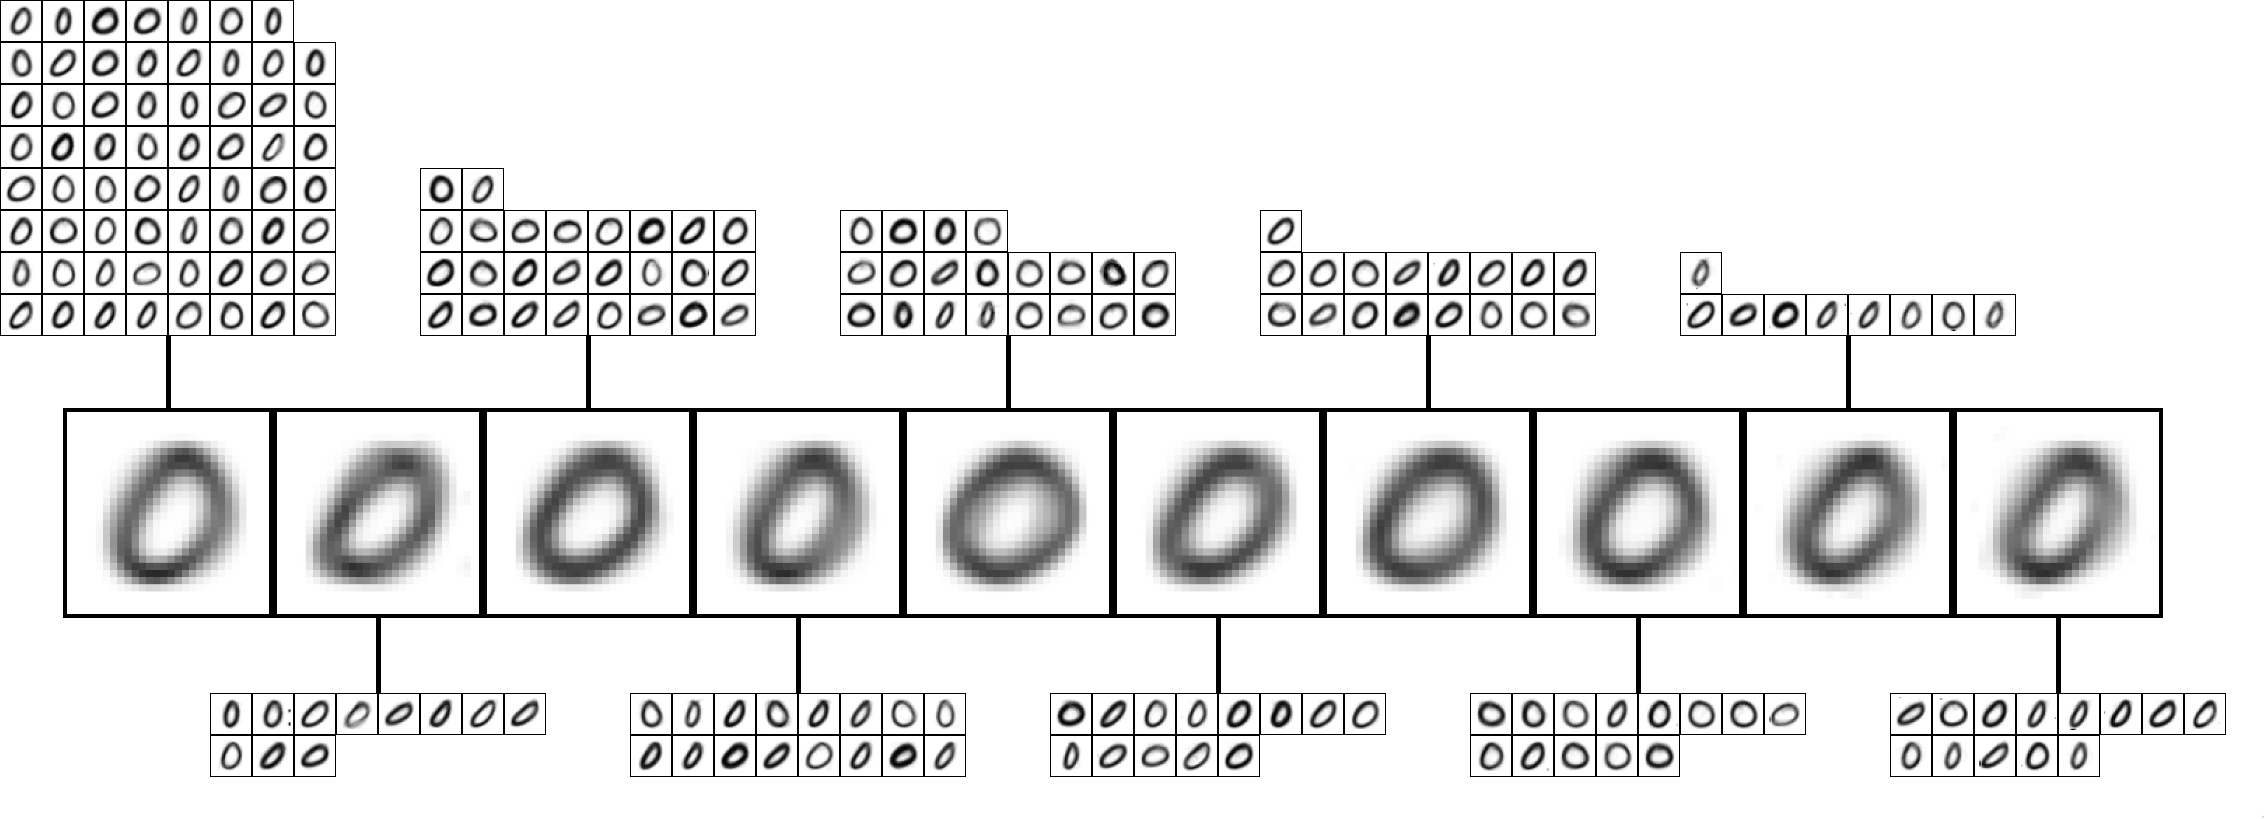
\includegraphics{figures/mnist.png}
  }
  \caption[Hierarchical clustering of MNIST-0 dataset]{Hierarchical clustering: Modes (representatives of the clusters) found in 2 iterations of Modal EM in GSPNs learned from MNIST-0 dataset. The smaller images correspond to the modes found in the first GSPN, the bigger ones correspond to the modes found in the second GSPN (learned from the modes from the first GSPN). Modes from the first GSPN are connected to their modes in the second GSPN. Source: \citet{Madeira2022}.}
  \label{fig:mnist}
\end{figure}

As noted in the paper, a limitation of this approach is that it tends to underrepresent high-density regions (large clusters) while overrepresenting low-density regions (small clusters) in the new dataset. To address this issue, one potential solution is to optimize for weighted log-likelihood in the structural and parametric learning algorithms. Another approach is to adjust the representation of models by over/undersampling them based on the density of their respective regions.

\section{Image segmentation}
\label{sec:exp:segmentation}

As another preliminary and visual investigation of the effectiveness of modal clustering on GSPNs, we performed some experiments with segmentation of the images depicted in Figure \ref{fig:segoriginals}.

\begin{figure}
  \centering

  \begin{minipage}{0.5\textwidth}
    \centering

    \scalebox{0.7}{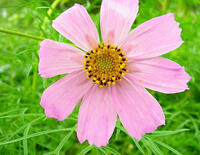
\includegraphics{figures/flower_200.jpg}}

    (a)
  \end{minipage}\begin{minipage}{0.5\textwidth}
    \centering

    \scalebox{0.7}{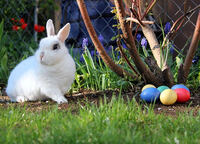
\includegraphics{figures/rabbit_200.jpg}}

    (b)
  \end{minipage}

  \vspace{0.5em}

  \begin{minipage}{0.5\textwidth}
    \centering

    \scalebox{0.7}{
\includegraphics{figures/tarsila3_200.jpg}}

    (c)
  \end{minipage}\begin{minipage}{0.5\textwidth}
    \centering

    \scalebox{0.7}{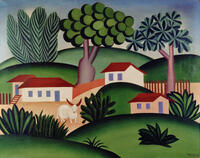
\includegraphics{figures/tarsila2_200.jpg}}

    (d)
  \end{minipage}

  \caption[Images used for segmentation (Flower, Easter Bunny, The Family, Landscape with Bull)]{Images used for segmentation. (a) Flower (200x155). (b) Easter Bunny (200x144). (c) Tarsila do Amaral's \emph{The Family} (200x158). (d) Tarsila do Amaral's \emph{Landscape with Bull} (200x158).}
  \label{fig:segoriginals}
\end{figure}

We generated datasets consisting of 5 variables by considering the RGB intensity values and $x$ and $y$ locations of each pixel from various images. The datasets were then used to learn GSPNs from data. We ran Modal EM starting from all the points in the dataset, finding the modes for which they converge. We considered that a cluster is formed by points that converge to the same mode. We then re-colored the image using the average color of the points in the cluster.

We experimented with different GSPNs by varying the minimum number of instances required for slicing in the learning process ($s$). Table \ref{tab:segstats} shows the number of nodes, network height and the number of clusters obtained for each GSPN when we vary $s$. One sees the great dependence between those quantities, as well as the quick increase in the number of modes when $s$ is smaller.

Figures \ref{fig:seg1} and \ref{fig:seg2} display a visual comparison of image segmentation by Modal EM in GSPNs and by the $k$-means algorithm as implemented by the scikit-learn library\footnote{Available at \url{https://scikit-learn.org}.}, where $k$ is set to the number of clusters identified by Modal EM trained with different $s$ hyperparameters.

Our results have shown satisfactory performance comparable to the widely-used $k$-means algorithm. However, visually, we observed that image segmentation using $k$-means with $k$ equivalent to the number of modes in the SPN yields more detailed segmentation results.

We conjecture that GSPN's slightly worse performance is due to a lack of fit to the model, which could be mitigated by changing the structure learning algorithm, performing fine-tuning of parameters or even using $k$-means solution as a initial model for refinements.

It is worth noting that image segmentation may not be the optimal application domain for SPNs, and also that GSPN modal clustering offers several advantages over traditional clustering techniques like $k$-means. It can effectively handle missing values, detect outliers based on probability thresholds, and easily scale up to handle more complex and high-dimensional domains.

\begin{table}
  \centering

  \begin{tabular}{crrrr}
    \toprule
    \bfseries Dataset   & \bfseries Parameter $s$ & \bfseries Nodes & \bfseries Height & \bfseries Clusters \\ \midrule
    Easter Bunny        & 20,000                  & 13              & 3                & 6                  \\
    Easter Bunny        & 15,000                  & 19              & 3                & 7                  \\
    Easter Bunny        & 10,000                  & 25              & 3                & 10                 \\
    Easter Bunny        & 5,000                   & 50              & 5                & 31                 \\
    Easter Bunny        & 2,000                   & 132             & 5                & 68                 \\
    Easter Bunny        & 500                     & 528             & 7                & 398                \\
    Easter Bunny        & 200                     & 1,267           & 9                & 676                \\ \midrule
    Flower              & 20,000                  & 13              & 3                & 2                  \\
    Flower              & 15,000                  & 19              & 3                & 5                  \\
    Flower              & 10,000                  & 25              & 3                & 8                  \\
    Flower              & 5,000                   & 61              & 3                & 27                 \\
    Flower              & 2,000                   & 155             & 5                & 79                 \\
    Flower              & 500                     & 595             & 5                & 228                \\
    Flower              & 200                     & 1,457           & 7                & 609                \\ \midrule
    The Family          & 20,000                  & 13              & 3                & 4                  \\
    The Family          & 15,000                  & 25              & 3                & 5                  \\
    The Family          & 10,000                  & 31              & 3                & 8                  \\
    The Family          & 5,000                   & 61              & 3                & 19                 \\
    The Family          & 2,000                   & 163             & 3                & 43                 \\
    The Family          & 500                     & 603             & 7                & 187                \\
    The Family          & 200                     & 1,504           & 7                & 555                \\ \midrule
    Landscape with Bull & 20,000                  & 13              & 3                & 6                  \\
    Landscape with Bull & 15,000                  & 25              & 3                & 12                 \\
    Landscape with Bull & 10,000                  & 31              & 3                & 15                 \\
    Landscape with Bull & 5,000                   & 55              & 3                & 24                 \\
    Landscape with Bull & 2,000                   & 145             & 3                & 38                 \\
    Landscape with Bull & 500                     & 563             & 7                & 255                \\
    Landscape with Bull & 200                     & 1,427           & 7                & 508                \\
    \bottomrule
  \end{tabular}

  \caption[Information about SPNs learned for image segmentation]{Information about SPNs learned for image segmentation.}
  \label{tab:segstats}
\end{table}

\newcommand{\segfigrow}[3]{
  \begin{minipage}{0.15\textwidth}
    \centering
    $s = #2$\\$k = #3$
  \end{minipage}    &
  \begin{minipage}{0.2\textwidth}
    \centering
    \scalebox{0.37}{\includegraphics{figures/fixed_mem_recolored_#1_200_#2_0.300000.png}}
  \end{minipage} &
  \begin{minipage}{0.2\textwidth}
    \centering
    \scalebox{0.37}{\includegraphics{figures/k_#3_recolored_#1_200.png}}
  \end{minipage}
}

\begin{figure}[p]
  \centering

  \begin{tabular}{ccc}
     & \bfseries GSPN & \bfseries $k$-means \\
    \segfigrow{flower}{20000}{2}            \\ \\
    \segfigrow{flower}{10000}{8}            \\ \\
    \segfigrow{flower}{2000}{79}            \\ \\
    \segfigrow{flower}{500}{228}            \\
  \end{tabular}

  \vspace{0.5em}

  (a)

  \vspace{2em}

  \begin{tabular}{ccc}
     & \bfseries GSPN & \bfseries $k$-means \\
    \segfigrow{rabbit}{20000}{6}            \\ \\
    \segfigrow{rabbit}{10000}{10}           \\ \\
    \segfigrow{rabbit}{2000}{68}            \\ \\
    \segfigrow{rabbit}{500}{398}            \\
  \end{tabular}

  \vspace{0.5em}

  (b)

  \caption[Image segmentation using GSPNs vs. $k$-means (Flower and Easter Bunny)]{Image segmentation using GSPNs vs. $k$-means. (a) Flower. (b) Easter Bunny.}
  \label{fig:seg1}
\end{figure}

\begin{figure}[p]
  \centering

  \begin{tabular}{ccc}
     & \bfseries GSPN & \bfseries $k$-means \\
    \segfigrow{tarsila3}{20000}{4}          \\ \\
    \segfigrow{tarsila3}{10000}{8}          \\ \\
    \segfigrow{tarsila3}{2000}{43}          \\ \\
    \segfigrow{tarsila3}{500}{187}          \\
  \end{tabular}

  \vspace{0.5em}

  (a)

  \vspace{2em}

  \begin{tabular}{ccc}
     & \bfseries GSPN & \bfseries $k$-means \\
    \segfigrow{tarsila2}{20000}{6}          \\ \\
    \segfigrow{tarsila2}{10000}{15}         \\ \\
    \segfigrow{tarsila2}{2000}{38}          \\ \\
    \segfigrow{tarsila2}{500}{255}          \\
  \end{tabular}

  \vspace{0.5em}

  (b)

  \caption[Image segmentation using GSPNs vs. $k$-means (The Family and Landscape with Bull)]{Image segmentation using GSPNs vs. $k$-means. (a) The Family. (b) Landscape with Bull.}
  \label{fig:seg2}
\end{figure}
